\documentclass{report}

\usepackage[ngerman]{babel}
\usepackage[utf8]{inputenc}
\usepackage[T1]{fontenc}
\usepackage{hyperref}
\usepackage{csquotes}
\usepackage{float}
\usepackage{caption}
\usepackage{graphicx}

\usepackage[
    backend=biber,
    style=apa,
    sortlocale=de_DE,
    natbib=true,
    url=false,
    doi=false,
    sortcites=true,
    sorting=nyt,
    isbn=false,
    hyperref=true,
    backref=false,
    giveninits=false,
    eprint=false]{biblatex}
\addbibresource{../references/bibliography.bib}


\title{KI und Datenschutz}
\author{Marina Brun}
\date{\today}

\parindent=0pt

\begin{document}

\maketitle



\tableofcontents

\chapter{Einleitung}

\section{Was ist KI?}

Das Thema Künstliche Intelligenz gewinnt in der sich digitalisierenden Welt immer mehr an Bedeutung. Sie bietet viele neue Möglichkeiten, jedoch hat man einige Bedenken bezüglich des Datenschutzes und der Privatsphäre. Diese Probleme werde ich erläutern und auf sie eingehen.

\vspace{2mm}Doch um das zu verstehen, ist es wichtig die Grundlagen zu wissen. Was ist eigentlich KI? Die künstliche Intelligenz ist die Fähigkeiten die Computer haben, Aufgaben zu erledigen, für die man eigentlich das Denken eines Menschen benötigt. Es ist die Fähigkeit von Maschinen Daten zu analysieren, Entscheidungen zu treffen und verschiedene Muster zu erkennen. Für diese Aufgaben umfasst die KI verschiedene Technologien und Methoden. Zu diesen gehören unter anderem das maschinelle Lernen, das neuronale Netzwerk und die Datenanalyse.

\vspace{2mm}Maschinelles Lernen ist ein Teilbereich der KI, welcher sich auf Algorithmen und Modelle konzentriert und es Maschinen ermöglicht, aus Daten zu lernen und Entscheidungen zu treffen, ohne vorher dafür programmiert werden zu müssen. Es ermöglicht dem Computer aus Erfahrungen zu lernen, sich selbstständig zu verbessern und seine Fähigkeiten zu verfeinern.

\vspace{2mm}Unter dem Begriff neuronale Netzwerke versteht man die Algorithmen die auf dem Konzept des menschlichen Gehirn basieren, welche die Erkennung komplexer Muster ermöglicht.  Es ahmt sozusagen das menschliche Hirn nach.

\vspace{2mm}Die Datenanalyse besteht darin grosse Mengen an Daten zu verarbeiten, um danach daraus wichtige Erkenntnisse zu gewinnen.

\section{Wie wird KI trainiert?}

Das Trainieren einer künstlichen Intelligenz wird in drei Schritte unterteilt. Im ersten Schritt werden viele Daten in ein Computersystem eingespeist. Dadurch lernt das System bessere Vorhersagen zu treffen und die Genauigkeit der Antworten immer zu verfeinern. Das wird durch das maschinelle Lernen erreicht. So bringt man der Software bei, Merkmale in einem Bild zu erkennen. Mit der Zeit werden die Vermutungen immer genauer, bis man sie nicht mehr verbessern kann. Darum werden riesige Mengen an Daten eingespeist. Wenn man jetzt zum Beispiel ein Algorithmus für Gesichtserkennung entwickeln will, muss man das Modell mit Daten von verschiedenen Gesichtern füttern. 

\vspace{2mm}Im zweiten Schritt wird er Validierungstest durchgeführt. Dieser bewertet die entwickelten Modelle beim analysieren von Daten, die sie vorher noch nicht kannten. Dadurch kann man feststellen, ob das Training fortgesetzt werden kann oder man es irgendwie verändern muss. 

\vspace{2mm}Das Testen der KI ist der dritte Schritt des Trainings. Man gibt ihr einen Datensatz ohne Tags und Ziele, welche ihr bis jetzt bei der Interpretation der Daten nur geholfen hat. Wenn sie möglichst genaue Entscheidungen trifft, ist die bereit in Betrieb zu gehen. Man muss jedoch überprüfen ob die künstliche Intelligenz auch eine 100 prozentige Genauigkeit erreicht.

\begin{figure}[h]
    \centering
    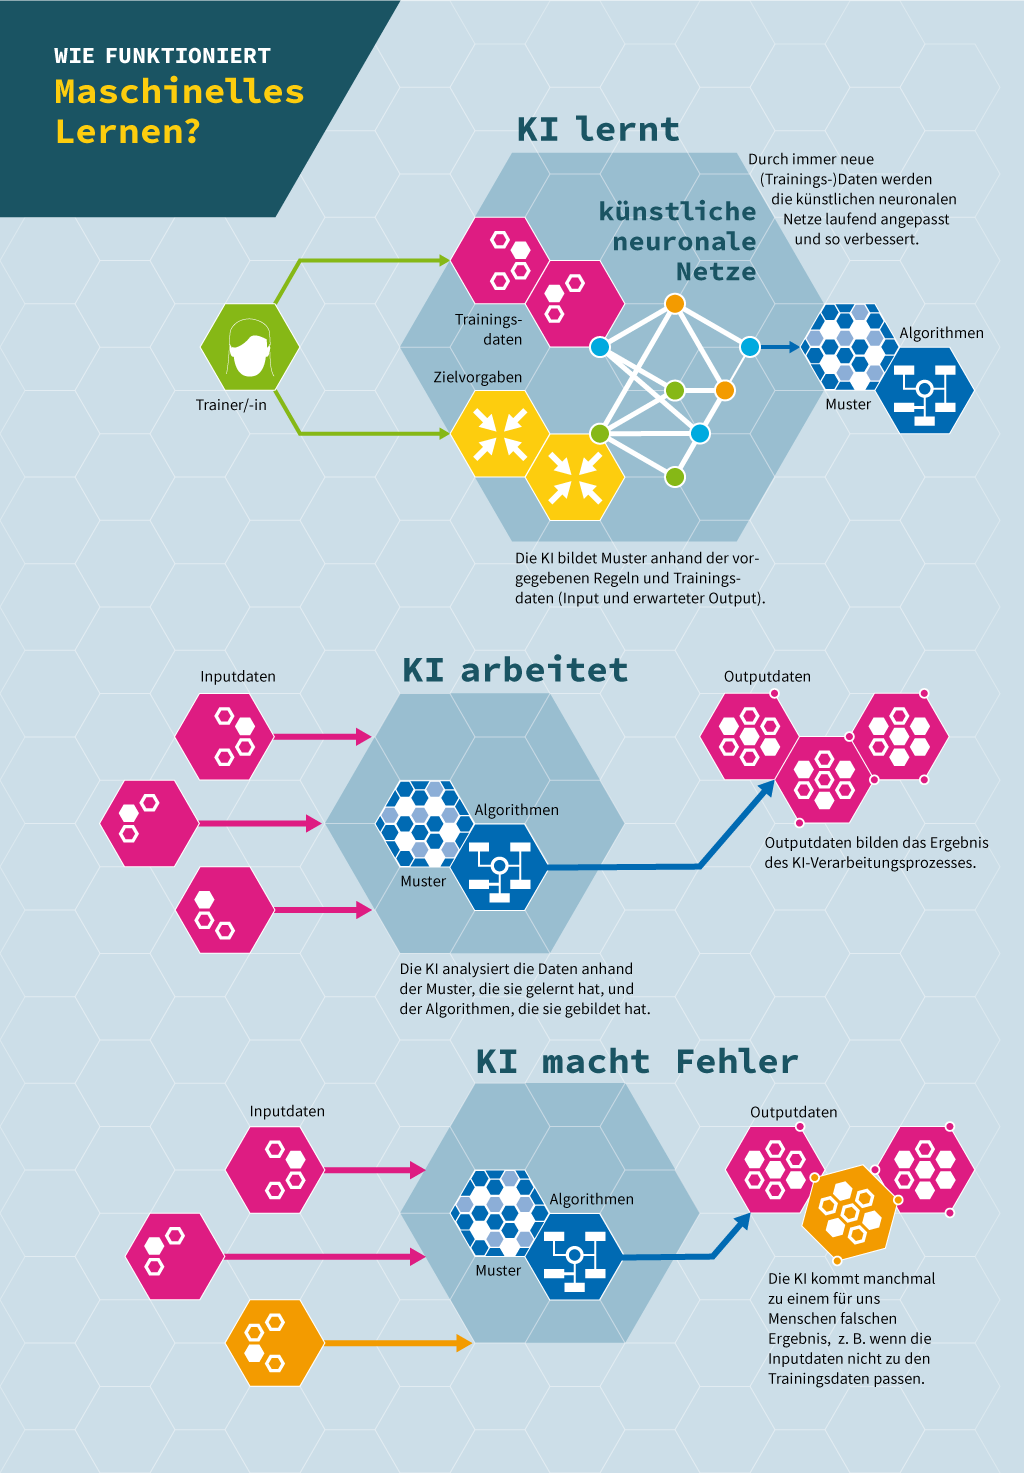
\includegraphics[width=0.5\textwidth]{training.png}
    %\caption{Ein erstes Bild}
    %\label{fig:meme}
    \end{figure}

\chapter{Datenschutz und Privatsphäre}

\section{Welche Bedenken gibt es hinslichtlich des Datenschutzes und der Privatsphäre in KI-Anwendung?}

Auch wenn die künstliche Intelligenz in der heutigen Gesellschaft viele Vorteile hat, gibt es einige Probleme bezüglich des Datenschutzes und der Privatsphäre.

\vspace{2mm}Der Datenschutz schützt die personenbezogenen Daten vor unerlaubten Zugriff und vor Missbrauch. In der digitalen Welt, wo viele Unternehmen und Organisationen die Daten einer Person verwenden, um Entscheidungen zu treffen oder personalisierte Werbungen und Dienstleistungen anzubieten, spielt der Datenschutz eine wichtige Rolle. Er ist wichtig, um das Vertrauen der Menschen aufrechtzuerhalten. Man entwickelte Datenschutzgesetze und Richtlinien, die festlegen, wie Daten gesammelt, gespeichert, verarbeitet und weitergegeben werden dürfen. Die einzelnen Nutzer haben auch das Recht ihre Daten zu korrigieren und zu löschen.

\vspace{2mm}Eines der grössten Anliegen ist der Schutz der personenbezogenen Daten. Da KI -Systeme grosse Mengen an Daten verarbeiten, können diese persönliche Daten enthalten. Wenn diese nicht genug geschützt sind, kann es passieren, dass sie durch Cyberangriffe oder Sicherheitslücken in falsche Hände geraten. Dadurch können Hacker auf diese Daten zugreifen und Identitätsdiebstahl oder finanziellen Betrug begehen. Diese Daten können auch für gezielte Betrugsversuche ausgenutzt werden. Kriminelle können durch betrügerische Aktivitäten sensible Informationen abfangen und ausnutzen. Auch in grossen Unternehmen kann der Zugriff auf unbefugte Daten zu Schaden führen und das Vertrauen missbrauchen. KI-Algorithmen können Daten auf eine Weise analysieren und verwenden, die nicht mit den Erwartungen der betroffenen Person übereinstimmen. Sowas kann passieren, wenn Daten ohne ausreichende Zustimmung oder Transparenz gesammelt und genutzt werden. Zum Beispiel könne solche Algorithmen Informationen aus den sozialen Medien nehmen, um Profile zu erstellen, ohne das die betroffene Person davon weiss oder sie zugestimmt hat. Wenn KI-Systeme auf persönliche Daten trainiert sind, können diese unbewusst, schon bestehende Vorurteile oder Diskriminierungen, verstärkt widergeben. Wenn die Trainingsdaten voreingenommen sind, werden die Ergebnisse der KI genauso voreingenommen widergespiegelt. Auch Sprachassistenten wie «Google Home» oder «Amazon Echo» werden zu einem Problem. Sie können Konversationen oder Situationen aufnehmen, auch wenn dies nicht von den betroffenen Leuten beabsichtigt wurde. Das ist sehr bedenklich in Bezug auf den Datenschutz. Man kann die Datenschutzfolgenabschätzung gar nicht beeinflussen, da der Algorithmus selbst entscheidet.


\begin{figure}[h]
    \centering
    
\includegraphics[width=0.8\textwidth]{datenschutz.jpg}
    %\caption{Ein erstes Bild}
    %\label{fig:meme}
    \end{figure}


    \chapter{Fazit}

    Insgesamt werden einem durch die künsltiche Intelligenz viele Vorteile geboten. Sie analysiert grosse Mengen an Daten und wodruch sie wertvolle Erkentnisse gewinnt. Trotzdem gibt es viele Bedenken hinsichtlich des Datenschutzes und der Privatsphäre, weil sie zum einen persönliche Informationen verarbeitet welche bei einem Mangel an Datenschutz zu Betrug oder Identitätsdiebstahl führen kann, und zum anderen aber auch Gespräche ungewollt aufzeichnet. Um solchen Risiken aus dem Weg zu gehen, sind Datenschutzrichtlinien streng zu beachten, damit man das Vertrauen der Nutzer nicht schädigt und ethische Herausforderungen bewältigen kann.




\nocite{*}

\printbibliography

\end{document}

